\documentclass[11pt, a4paper, leqno]{article}
\usepackage{a4wide}
\usepackage[T1]{fontenc}
\usepackage[utf8]{inputenc}
\usepackage{float, afterpage, rotating, graphicx}
\usepackage{epstopdf}
\usepackage{longtable, booktabs, tabularx}
\usepackage{fancyvrb, moreverb, relsize}
\usepackage{eurosym, calc}
\usepackage{chngcntr}
\usepackage{amsmath, amssymb, amsfonts, amsthm, bm}
\usepackage{caption}
\usepackage{mdwlist}
\usepackage{adjustbox}
\usepackage{xfrac}
\usepackage{setspace}
\usepackage[dvipsnames]{xcolor}
\usepackage{subcaption}
\usepackage{minibox}
\usepackage{graphicx}
% \usepackage{pdf14} % Enable for Manuscriptcentral -- can't handle pdf 1.5
% \usepackage{endfloat} % Enable to move tables / figures to the end. Useful for some
% submissions.

\usepackage[
    natbib=true,
    bibencoding=inputenc,
    bibstyle=authoryear-ibid,
    citestyle=authoryear-comp,
    maxcitenames=3,
    maxbibnames=10,
    useprefix=false,
    sortcites=true,
    backend=biber
]{biblatex}
\AtBeginDocument{\toggletrue{blx@useprefix}}
\AtBeginBibliography{\togglefalse{blx@useprefix}}
\setlength{\bibitemsep}{1.5ex}
\addbibresource{../paper/refs.bib}


\usepackage[unicode=true]{hyperref}
\hypersetup{
    colorlinks=true,
    linkcolor=black,
    anchorcolor=black,
    citecolor=NavyBlue,
    filecolor=black,
    menucolor=black,
    runcolor=black,
    urlcolor=NavyBlue
}


\widowpenalty=10000
\clubpenalty=10000

\setlength{\parskip}{1ex}
\setlength{\parindent}{0ex}
\setstretch{1.5}



\begin{document}

\title{Climate Shocks and Resource Management: Exploring Decision Dynamics in Common Pool Extraction \thanks{Sushmita Saha, 50066526, University of Bonn. Email: \href{mailto:s67ssaha@uni-bonn.de}{\nolinkurl{s67ssaha[at] uni-bonn [dot] de}}.}}

\author{Sushmita Saha}
\date{}
\maketitle
\begin{abstract}
This study investigates the interaction between perceptions of extraction behaviours and awareness of climate shocks across diverse cultural contexts, focusing on India, Indonesia, and Germany. Utilizing Qualtrics as an online survey methodology, data was collected to elucidate the nuances in attitudes and awareness regarding resource extraction and its environmental implications. The study explores variations in perceptions across the three countries, shedding light on cultural influences that shape attitudes towards sustainable resource management and climate resilience. Findings reveal distinct patterns in how individuals from different cultural backgrounds perceive extraction behaviours and their associated climate impacts. Moreover, the study provides insights into the level of awareness regarding climate shocks and their implications for environmental sustainability. By uncovering these cross-cultural variations, this research contributes to a deeper understanding of global perspectives on resource management and climate resilience, offering valuable implications for policy-making and cross-cultural environmental education initiatives.
\end{abstract}



\clearpage
\section{Introduction}\label{sec:introduction}
 % (fold)

Over the last 50 years, there has been a significant reconsideration of how individuals approach decision-making related to the extraction of resources from shared pools, such as forests, fisheries, and water bodies  \href{https://api.semanticscholar.org/CorpusID:54717731}{(Ghate, Ghate, and Ostrom, 2013)}. In the coming decades, the deterioration of natural resources is expected to speed up due to factors like climate change, unchecked population growth, and shifts in demand patterns in both developing and developed countries. However, the impact of scarcity on human behaviour continues to be a subject of ongoing research \href{https://api.semanticscholar.org/CorpusID:155012795}{(Gatiso, Vollan, and Nuppenau, 2015)}. 

In recent years, climate change has increasingly become a focal point for both researchers and policymakers. The \href{https://doi.org/10.59327/IPCC/AR6-9789291691647.001}{ Intergovernmental Panel on Climate Change (IPCC) (2023)}.
 clearly outlines the severe impacts of human-induced climate change on ecological and societal structures, emphasizing the urgent need for global efforts in mitigation and adaptation. The report highlights the rise in frequency and severity of climate-related events, such as extreme weather, and their negative effects on biodiversity, food security, and water resources.

Considering these increasing risks, our study investigates the effects of anticipated climate shocks on decision-making in common pool resource extraction diverging away from prior research focusing on prevailing scarcity, identifying a positive relationship between antisocial behaviour and long-term scarcity exposure  \href{https://doi.org/10.1016/j.jpubeco.2014.07.007}{(Prediger, Vollan, and Herrmann, 2014)}. Specifically, we investigate how the perceived probability of climate shocks influences individuals' decisions to extract resources. 


 We hypothesize that an elevated risk will lead to higher extraction rates, driven by a lower expected future value of the resource. Furthermore, our investigation seeks to determine whether individuals with pro-environmental attitudes, as identified by the Environmental Attitudes Inventory (EAI) \href{https://doi.org/10.1016/j.jenvp.2009.09.001}{(Milfont and Duckitt, 2010)}, demonstrate lower resource extraction rates compared to their counterparts.

Our methodology involves an online survey conducted across India, Indonesia, and Germany to gauge how perceptions of different extraction behaviours and awareness of climate shocks vary between countries.

Our findings reveal a significant increase in extraction rates under high-risk climate shocks compared to lower- and no-risk scenarios, highlighting the significant role that the probability of climate shocks plays in resource management decisions. Additionally, our analysis reveals that individuals who hold pro-environmental values, as identified through the Environmental Attitude Inventory (EAI), tend to engage in reduced extraction activities under normal conditions. However, this tendency does not persist in scenarios where a climate shock is anticipated. This observation aligns with the insights provided by \href{https://doi.org/10.1111/j.1559-1816.1996.tb01100.x}{ Hine and Gifford (1996)}, who noted that the presence of uncertainty tends to diminish pro-environmental behaviours. 

The paper has the following structure. In the next section, (i) study design, where we explain the source of our data, and (ii) experimental design, which sets the hypotheses of our groundwork. Section 4 discusses the analysis and our results on behavioural outcomes related to climate shock and its anticipation. Section 5 concludes, followed by a list of references.




 \section{Study Design} % (fold)
\label{Study Design}
An online survey was conducted among participants residing in Germany, Indonesia, and India. To be eligible to participate in the study, respondents had to reside in one of these countries and be at least 18 years old. The data collection was carried out in January 2024, and the survey was scripted in the survey software Qualtrics. 

The survey distributed amongst participants included questions aiming to evaluate to what extent people understand what would be the optimal strategy in the game. Moreover, we included the short 24-item version of the Environmental Attitudes Inventory \href{https://api.semanticscholar.org/CorpusID:59149978}{ (Milfont, Duckitt and Wagner, 2010)}, which is a measure to evaluate the structure of environmental attitudes \href{https://doi.org/10.1016/j.jenvp.2009.09.001}{(Milfont and Duckitt, 2010)}. For later analysis, we use the Generalized Environmental Attitude mean score mentioned in the paper by \href{https://doi.org/10.1016/j.jenvp.2009.09.001}{(Milfont and Duckitt, 2010)}. To then further categorize people as pro-environmental or not pro-environmental we performed a median split.
Questions from \href{https://api.semanticscholar.org/CorpusID:261216513}{Andre et al. (2022)} were taken and adapted to climate shocks to measure climate change concern and scepticism. Global Preference Survey questions were included to measure risk aversion, patience, positive and negative reciprocity, altruism and trust. Only the qualitative measures were used for this. 
In addition to these measures, the survey also integrated questions aimed at understanding participants' perceptions and experiences of climate shocks, their beliefs regarding the impact of individual and collective actions on environmental conservation, and various demographic factors.
\medskip

The online survey also included a section where subjects were asked to evaluate different behaviours of resource extraction in the context of a high and a low risk for a climate shock. Behaviours were rated in terms of sustainability, morals, how one would behave, how they think others would behave and how they think other people think people should behave.

In a nutshell, the survey aims to gather information on individuals' awareness, attitudes, and behaviours related to tree cutting, environmental conservation, climate shocks, and pro-environmental actions. It explores awareness of climate-related activities, concerns about environmental impacts, and perceptions of climate-related shocks. Overall, the survey aims to provide a holistic view of participants' environmental consciousness and engagement.

\section{Experimental Design} % (fold)
\label{sec:Data and Variables}
In one section of the survey participants were asked to evaluate the behaviours of three individuals A, B, and C where Person A demonstrated the most environmentally sustainable actions, and Person C the least. This assessment was conducted twice, once under a scenario of low risk for a climate shock and again under high risk. Evaluations
focused on sustainability, morals, how one would behave, how they think others would behave and how they think other people think people should behave. Following this, we ran an independent t-test. 

In an independent t-test, we compare the means of two independent groups to determine if there is a significant difference between them. The assumption is that the samples are independent, meaning that the observations in one group are not related to the observations in the other group.
In our case, we are comparing the means of two independent groups: the low-risk and high-risk groups for each combination of person and category. Each person has two groups (low and high risk), and for each person, we are conducting separate t-tests for each category, which helped us frame the following hypotheses:

\medskip
\begin{adjustbox}{minipage=.7\textwidth,margin=0pt \smallskipamount,center}
    \itshape \noindent \textbf{H0}: There is no significant difference in the average ratings between low and high climate risk for each category for all persons (A, B, C).
    
    \itshape \noindent \textbf{H1}: There is a statistically significant difference in the average ratings between low and high climate risk for at least one person.
\end{adjustbox}
\medskip

The survey also had questions from the short 24-item version of the Environmental Attitudes Inventory \href{https://api.semanticscholar.org/CorpusID:59149978}{ (Milfont, Duckitt and Wagner, 2010)} and the Global Preference Survey \href{https://api.semanticscholar.org/CorpusID:34720979}{  (Falk et al., 2018)}. The last two adopted survey questions are then used to measure personal attitudes and perceptions towards environmentalism, and their preferences with respect to altruism, reciprocity, time preference, risk preference and trust. All these variables we believe to be important exogenous factors influencing individual and group extraction behaviour in the experiment, which led us to our second hypothesis:

\medskip
\begin{adjustbox}{minipage=.7\textwidth,margin=0pt \smallskipamount,center}
    \itshape \noindent \textbf{H2}: Subjects categorized as pro-environmental according to the Environmental Attitudes Inventory (EAI) are comparatively more experienced with climate shock.
\end{adjustbox}
\medskip

This exploratory study was done to understand how people living in different countries with varying degrees of climate shock risks may have different perceptions and behaviour
towards pro-environmentalist behaviour. 



 \section{Results and Discussions} % (fold)
\label{sec:Results & Discussions}

\subsubsection{Judgment of Described Behavior}


In this section, participants were presented with two scenarios - (i) low risk, (ii) and high risk, related to extracting natural resources, specifically trees, in a hypothetical location. The scenarios considered varying probabilities of resource loss due to climate shocks. 
Participants were asked to evaluate the behaviours of three individuals A, B, and C where Person A demonstrated the most environmentally sustainable actions, and Person C the least. This assessment was conducted twice, once under a scenario of low risk for a climate shock and again under high risk. Evaluations focused on sustainability, morals, how one would behave, how they think others would behave and how they think other people think people should behave.

\begin{figure}[H]
  \centering
  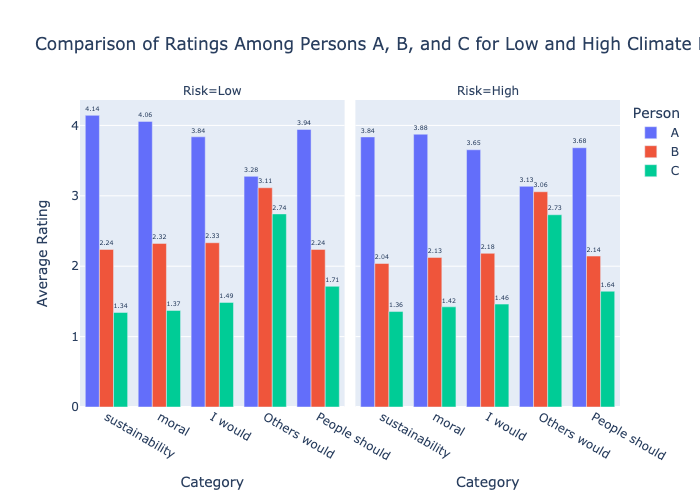
\includegraphics[width=1.0\textwidth]{../bld/Fig1.png} 
  \caption{Perceived Environmental Responsibility: Self-Assessment vs. Social Perception Amid Climate Risk}
\end{figure}


\noindent In Figure 1, a notable trend emerged where participants rated themselves as relatively environmentally friendly, indicating a preference for behaving similarly to Person A, who is characterized by environmentally sustainable actions. Conversely, they perceived others as more likely to exhibit behaviours akin to Persons B and C, suggesting a less environmentally friendly approach. When assessing behaviours in terms of sustainability, morality, and societal expectations (how they think other people think people should behave), the ratings were relatively consistent across these dimensions, indicating a general agreement on what constitutes environmentally responsible behaviour.

\noindent Interestingly, the comparison between scenarios with low and high risk for a climate shock revealed only slight differences in responses. This suggests a stable perception of environmental behaviours, regardless of the varying risk levels of climate shocks.


The findings from Figure 2 revealed a notable consistency in participant ratings across both high and low-risk scenarios. Surprisingly, respondents assigned nearly identical ratings regardless of the varying levels of environmental risk. This unexpected parallelism suggests a robust and consistent trend in participants' evaluations of behavior related to natural resource extraction, irrespective of the perceived likelihood of climate shocks. This finding underscores the importance of understanding the underlying factors influencing participants' judgment and highlights the need for further investigation into the stability of these assessments in different environmental contexts.


\subsection{Descriptive Statistics}

\subsubsection{T-test}

In analyzing the results of our survey on judgments of behaviour in scenarios involving resource extraction and climate risk, several noteworthy patterns emerge. Our focus was on evaluating differences in average ratings between low and high climate risk scenarios for each individual (Persons A, B, and C) across various categories including sustainability, morality, personal behaviour alignment, perceived societal behaviour alignment, and societal expectations.


\begin{figure}[H]
  \centering
  \includegraphics[width=1.0\textwidth]{../bld/Fig2.png} 
  \caption{T-test}
\end{figure}

Figure 2 reveals intriguing nuances of our hypothesis with the help of a heatmap. For Person A, our analysis revealed a statistically significant difference in sustainability ratings between low and high climate risk scenarios, supporting our hypothesis that climate risk influences perceptions of sustainability in resource extraction practices. However, this significance was not observed across other categories, indicating a more nuanced relationship between climate risk and moral judgments.


Conversely, for Person B, t-test results did not yield statistically significant differences in any category, suggesting a consistent perception of behaviour irrespective of environmental conditions. This finding challenges our initial expectations and emphasizes the need for further exploration into the factors influencing judgment in resource extraction scenarios.

Furthermore, the consistent t-test results for Person C across both low and high-climate risk scenarios highlight a fixed perception of behaviour, regardless of environmental context. While this lack of variability may indicate a stable judgment, it also raises questions about the underlying assumptions and biases shaping perceptions of sustainability and morality.

In conclusion, our t-test analysis provides valuable insights into the complex interplay between individual behaviour, societal perceptions, and environmental risk. These findings underscore the importance of considering multiple factors when evaluating judgments of behaviour in resource extraction scenarios and highlight avenues for future research in this domain.

\subsubsection{Environmental Score}

In one section of the survey, we included the short 24-item version of the Environmental Attitudes Inventory \href{https://api.semanticscholar.org/CorpusID:59149978}{ (Milfont, Duckitt and Wagner, 2010)}, which is a measure to evaluate the structure of environmental attitudes \href{https://doi.org/10.1016/j.jenvp.2009.09.001}{(Milfont and Duckitt, 2010)}.. The Generalized Environmental Attitude (GEA) mean score was computed as per the methodology outlined by \href{https://doi.org/10.1016/j.jenvp.2009.09.001}{Milfont and Duckitt, 2010}. To then further categorize people as pro-environmental or not pro-environmental we did a median split.

After reversing scores for certain items to ensure consistency, we calculated the GEA score by summing the responses across all items and dividing by the total number of items (24). The resulting GEA score provides an overarching measure of participants' environmental attitudes, with higher scores indicating stronger pro-environmental tendencies. 

To further analyze the data, respondents were categorized into two groups based on their GEA scores. A cutoff point of 4 on the Likert scale was utilized, with respondents scoring above 4 classified as pro-environmentalists and those scoring 4 or below categorized as not pro-environmentalists. This categorization allowed for a clearer distinction between individuals with varying degrees of agreement with pro-environmental statements.

\begin{figure} [h]
  \centering
  \includegraphics[width=1.0\textwidth]{../bld/Fig3.png} 
  \caption{Environmental attitudes across countries}
\end{figure}

As seen in Figure 3, the distribution of pro-environmentalists and not pro-environmentalists was examined across different geographic locations, including India, Germany, and Indonesia. Figure 3 illustrates the differences in environmental attitudes among respondents from these diverse regions.


Our analysis revealed notable variations in environmental attitudes across geographical locations. Specifically, a higher proportion of pro-environmentalists was observed among respondents from Indonesia compared to those from Germany and India. In Figure 6 we see that participants from India have been affected by the climate shock the most, but unfortunately, their percentage of pro-environmentalists is the lowest, as shown in Figure 3. This suggests the unawareness of the impact of climate shocks amongst the participants of India. 

These findings underscore the importance of considering regional differences in environmental attitudes when designing policies and interventions aimed at promoting environmental sustainability. 

.

 
\subsection{Further Analysis}

\subsubsection{Measuring Climate Change Skepticism}

In this segment, participants responded to a set of questions aimed to gauge individuals' beliefs regarding climate shocks \href{https://www.econtribute.de/RePEc/ajk/ajkdps/ECONtribute_101_2021.pdf}{(Falk, André, Boneva, and Chopra, 2021)}. The response options allowed participants to express varying degrees of concern, assessment of harm, and opinions on the origins of climate shocks, contributing to a comprehensive understanding of attitudes toward climate change.


\begin{figure} [h]
  \centering
  \includegraphics[width=1.0\textwidth]{../bld/Fig4.png} 
  \caption{Cross-country analysis}
\end{figure}

\noindent The analysis of responses, represented in Figure 3, revealed a striking consensus among participants from these diverse regions. A substantial majority across all countries expressed a shared belief that climate shocks are primarily a result of human activities. This alignment was further pronounced when considering opinions on the increased probability of climate shocks in recent times, with a noteworthy agreement that this heightened risk is predominantly attributable to human activities. These findings underscore a global convergence in acknowledging the significant impact of human actions on climate change, emphasizing the need for collective efforts to address and mitigate the consequences of environmental challenges.

\begin{figure} [h]
  \centering
  \includegraphics[width=1.0\textwidth]{../bld/Fig5.png} 
  \caption{Climate shock Experience}
\end{figure}

\noindent In Figure 6 we see that Indians had the highest rate of experiencing climate-related shocks or extreme weather events among the surveyed participants. This suggests that India might be more prone to such events or that a larger portion of the population has been affected by them compared to Indonesia and Germany.

\noindent However, despite experiencing fewer climate-related shocks, Indonesians expressed a greater level of worry about these events compared to their Indian counterparts. This discrepancy in concern might be attributed to various factors, including differences in socioeconomic conditions, geographical vulnerabilities, and cultural attitudes towards climate change.

\noindent For instance, while India's diverse socioeconomic landscape may result in varying levels of concern among its population, Indonesia's susceptibility to specific types of climate-related events, such as tropical storms and rising sea levels, could heighten awareness and worry despite lower exposure rates.

\noindent These findings underscore the complex interplay between direct experiences, perceived risks, and societal attitudes towards climate change. They highlight the importance of considering multiple factors, including socioeconomics, geography, and culture, when interpreting survey data related to climate impacts and public attitudes.

 

\section{Conclusion} % (fold)
\label{sec:Conclusion}
In conclusion, our study demonstrates how anticipated climate shocks significantly impact individual resource extraction behaviour in common pool resource settings, with participants exhibiting increased extraction rates when anticipating high climate risk, prioritizing short-term gains over long-term sustainability. This highlights the complexity of decision-making in uncertain conditions, where pro-environmental incentives weaken in the face of anticipated climate shocks.

Our findings underscore the importance of considering psychological and behavioural factors alongside economic and environmental aspects in devising mitigation and adaptation strategies for sustainable resource management amidst climate change. Additionally, our research highlights the need for adaptive decision-making processes and stresses the role of understanding human behaviour in fostering a resilient and equitable future.

Furthermore, our study uncovered a noteworthy level of concern among participants in Indonesia, suggesting the influence of cultural and societal factors on perceptions and responses to similar experimental conditions in different geographical contexts. Future research endeavours could explore these dynamics further to contribute to a more comprehensive understanding of global phenomena and enhance the applicability of findings.

While our study confirms hypotheses regarding increased tree removal with heightened climate risk and the influence of pro-environmental attitudes on extraction behaviour, limitations such as sample size and lack of communication during experiments warrant further investigation. Future research could explore the effects of group dynamics and communication, as well as replicate the study in different cultural contexts, such as Indonesia, to gain deeper insights into these phenomena.

\clearpage
\clearpage
\setstretch{1}
\nocite{*}
% Print bibliography
%\printbibliography % For BibLaTeX
% \bibliographystyle{plain} % For BibTeX
% \bibliography{your_bibliography} % For BibTeX

\end{document}